\begin{figure}[ht]
    \centering
    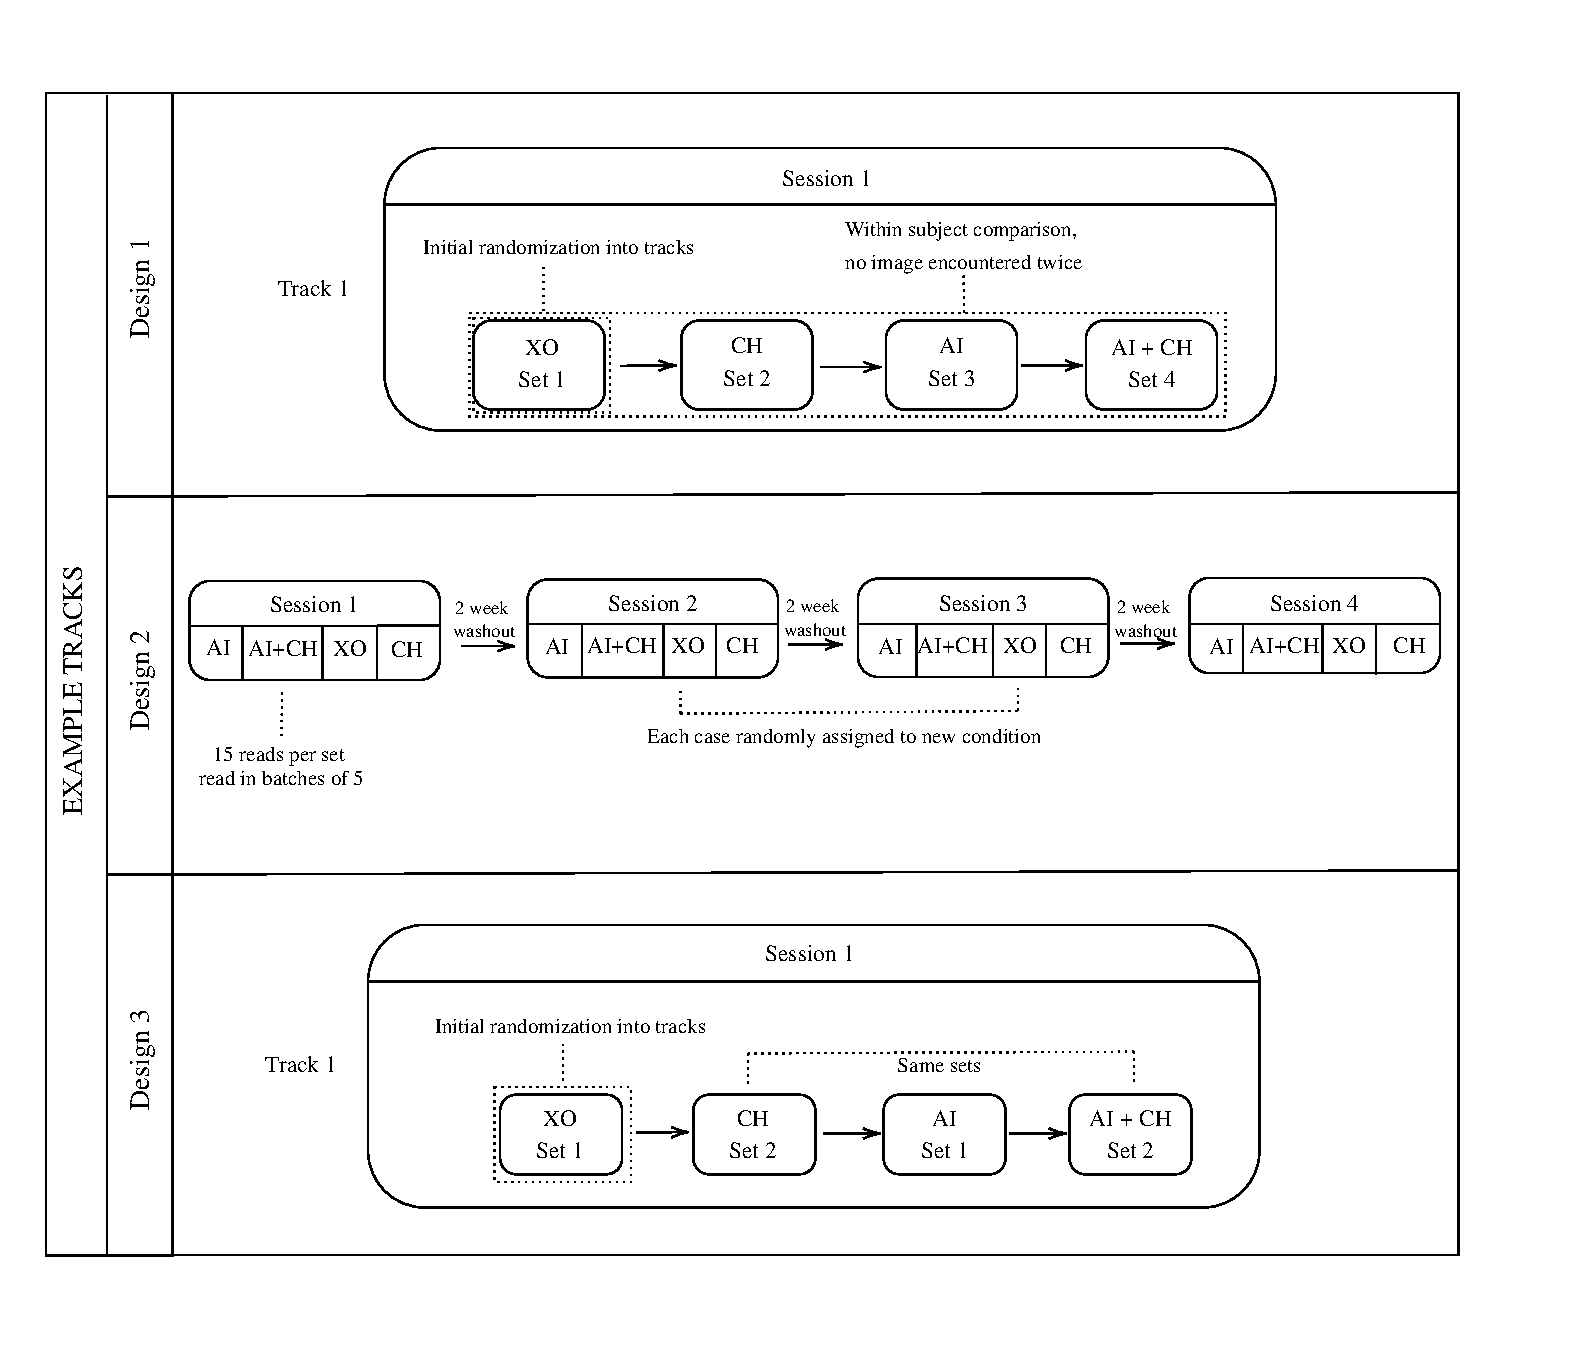
\includegraphics[width=0.8\textwidth]{images/designs.pdf}    
    \caption{Experimental designs}
    \label{fig:experiment_design}
\end{figure}

\begin{table}[ht]
    \centering
    \caption{Summary statistics\label{tab:summary_statistics}}
    \newcommand{\probtoplevelexpmean}{$0.233$}
\newcommand{\probtoplevelexpsd}{$0.290$}
\newcommand{\probtoplevelexpobs}{$36,280$}
\newcommand{\followuptoplevelexpmean}{$0.322$}
\newcommand{\followuptoplevelexpsd}{$0.467$}
\newcommand{\followuptoplevelexpobs}{$36,280$}
\newcommand{\devgttoplevelexpmean}{$0.223$}
\newcommand{\devgttoplevelexpsd}{$0.281$}
\newcommand{\devgttoplevelexpobs}{$36,280$}
\newcommand{\devaitoplevelexpmean}{$0.191$}
\newcommand{\devaitoplevelexpsd}{$0.169$}
\newcommand{\devaitoplevelexpobs}{$36,280$}
\newcommand{\aiaccuracytoplevelexpmean}{$0.261$}
\newcommand{\aiaccuracytoplevelexpsd}{$0.195$}
\newcommand{\aiaccuracytoplevelexpobs}{$36,280$}
\newcommand{\cordectoplevelexpmean}{$0.695$}
\newcommand{\cordectoplevelexpsd}{$0.460$}
\newcommand{\cordectoplevelexpobs}{$36,280$}
\newcommand{\activetimetoplevelexpmean}{$2.82$}
\newcommand{\activetimetoplevelexpsd}{$2.63$}
\newcommand{\activetimetoplevelexpobs}{$36,270$}
\newcommand{\clickstoplevelexpmean}{$45$}
\newcommand{\clickstoplevelexpsd}{$33$}
\newcommand{\clickstoplevelexpobs}{$36,270$}
\newcommand{\probradexpmean}{$0.250$}
\newcommand{\probradexpsd}{$0.304$}
\newcommand{\probradexpobs}{$180$}
\newcommand{\followupradexpmean}{$0.333$}
\newcommand{\followupradexpsd}{$0.473$}
\newcommand{\followupradexpobs}{$180$}
\newcommand{\devgtradexpmean}{$0.276$}
\newcommand{\devgtradexpsd}{$0.323$}
\newcommand{\devgtradexpobs}{$180$}
\newcommand{\devairadexpmean}{$0.205$}
\newcommand{\devairadexpsd}{$0.179$}
\newcommand{\devairadexpobs}{$180$}
\newcommand{\aiaccuracyradexpmean}{$0.281$}
\newcommand{\aiaccuracyradexpsd}{$0.215$}
\newcommand{\aiaccuracyradexpobs}{$180$}
\newcommand{\cordecradexpmean}{$0.678$}
\newcommand{\cordecradexpsd}{$0.469$}
\newcommand{\cordecradexpobs}{$180$}
\newcommand{\activetimeradexpmean}{$3.19$}
\newcommand{\activetimeradexpsd}{$3.24$}
\newcommand{\activetimeradexpobs}{$180$}
\newcommand{\clicksradexpmean}{$48$}
\newcommand{\clicksradexpsd}{$35$}
\newcommand{\clicksradexpobs}{$180$}
\newcommand{\probpooledaiexpmean}{$0.083$}
\newcommand{\probpooledaiexpsd}{$0.201$}
\newcommand{\probpooledaiexpobs}{$235,820$}
\newcommand{\followuppooledaiexpmean}{$0.122$}
\newcommand{\followuppooledaiexpsd}{$0.328$}
\newcommand{\followuppooledaiexpobs}{$235,820$}
\newcommand{\devgtpooledaiexpmean}{$0.085$}
\newcommand{\devgtpooledaiexpsd}{$0.205$}
\newcommand{\devgtpooledaiexpobs}{$235,820$}
\newcommand{\devaipooledaiexpmean}{$0.100$}
\newcommand{\devaipooledaiexpsd}{$0.135$}
\newcommand{\devaipooledaiexpobs}{$235,820$}
\newcommand{\aiaccuracypooledaiexpmean}{$0.117$}
\newcommand{\aiaccuracypooledaiexpsd}{$0.156$}
\newcommand{\aiaccuracypooledaiexpobs}{$235,820$}
\newcommand{\cordecpooledaiexpmean}{$0.882$}
\newcommand{\cordecpooledaiexpsd}{$0.323$}
\newcommand{\cordecpooledaiexpobs}{$235,820$}
\newcommand{\activetimepooledaiexpmean}{$2.82$}
\newcommand{\activetimepooledaiexpsd}{$2.63$}
\newcommand{\activetimepooledaiexpobs}{$235,755$}
\newcommand{\clickspooledaiexpmean}{$45$}
\newcommand{\clickspooledaiexpsd}{$33$}
\newcommand{\clickspooledaiexpobs}{$235,755$}
\newcommand{\probnormalexpmean}{$0.540$}
\newcommand{\probnormalexpsd}{$0.329$}
\newcommand{\probnormalexpobs}{$18,140$}
\newcommand{\followupnormalexpmean}{$0.528$}
\newcommand{\followupnormalexpsd}{$0.499$}
\newcommand{\followupnormalexpobs}{$18,140$}
\newcommand{\devgtnormalexpmean}{$0.423$}
\newcommand{\devgtnormalexpsd}{$0.323$}
\newcommand{\devgtnormalexpobs}{$18,140$}
\newcommand{\devainormalexpmean}{$0.245$}
\newcommand{\devainormalexpsd}{$0.204$}
\newcommand{\devainormalexpobs}{$18,140$}
\newcommand{\aiaccuracynormalexpmean}{$0.561$}
\newcommand{\aiaccuracynormalexpsd}{$0.279$}
\newcommand{\aiaccuracynormalexpobs}{$18,140$}
\newcommand{\cordecnormalexpmean}{$0.532$}
\newcommand{\cordecnormalexpsd}{$0.499$}
\newcommand{\cordecnormalexpobs}{$18,140$}
\newcommand{\activetimenormalexpmean}{$2.82$}
\newcommand{\activetimenormalexpsd}{$2.63$}
\newcommand{\activetimenormalexpobs}{$18,135$}
\newcommand{\clicksnormalexpmean}{$45$}
\newcommand{\clicksnormalexpsd}{$33$}
\newcommand{\clicksnormalexpobs}{$18,135$}
\newcommand{\probpooledexpmean}{$0.031$}
\newcommand{\probpooledexpsd}{$0.132$}
\newcommand{\probpooledexpobs}{$1,850,280$}
\newcommand{\followuppooledexpmean}{$0.077$}
\newcommand{\followuppooledexpsd}{$0.266$}
\newcommand{\followuppooledexpobs}{$526,060$}
\newcommand{\devgtpooledexpmean}{$0.032$}
\newcommand{\devgtpooledexpsd}{$0.133$}
\newcommand{\devgtpooledexpobs}{$1,850,280$}
\newcommand{\devaipooledexpmean}{$0.100$}
\newcommand{\devaipooledexpsd}{$0.135$}
\newcommand{\devaipooledexpobs}{$235,820$}
\newcommand{\aiaccuracypooledexpmean}{$0.117$}
\newcommand{\aiaccuracypooledexpsd}{$0.156$}
\newcommand{\aiaccuracypooledexpobs}{$235,820$}
\newcommand{\cordecpooledexpmean}{$0.979$}
\newcommand{\cordecpooledexpsd}{$0.144$}
\newcommand{\cordecpooledexpobs}{$1,850,280$}
\newcommand{\activetimepooledexpmean}{$2.82$}
\newcommand{\activetimepooledexpsd}{$2.63$}
\newcommand{\activetimepooledexpobs}{$1,849,770$}
\newcommand{\clickspooledexpmean}{$45$}
\newcommand{\clickspooledexpsd}{$33$}
\newcommand{\clickspooledexpobs}{$1,849,770$}

\newcommand{\probtopleveldomean}{$0.214$}
\newcommand{\probtopleveldosd}{$0.287$}
\newcommand{\probtopleveldoobs}{$13,440$}
\newcommand{\followuptopleveldomean}{$0.277$}
\newcommand{\followuptopleveldosd}{$0.448$}
\newcommand{\followuptopleveldoobs}{$13,440$}
\newcommand{\devgttopleveldomean}{$0.218$}
\newcommand{\devgttopleveldosd}{$0.290$}
\newcommand{\devgttopleveldoobs}{$13,440$}
\newcommand{\devaitopleveldomean}{$0.201$}
\newcommand{\devaitopleveldosd}{$0.171$}
\newcommand{\devaitopleveldoobs}{$13,440$}
\newcommand{\aiaccuracytopleveldomean}{$0.260$}
\newcommand{\aiaccuracytopleveldosd}{$0.193$}
\newcommand{\aiaccuracytopleveldoobs}{$13,440$}
\newcommand{\cordectopleveldomean}{$0.736$}
\newcommand{\cordectopleveldosd}{$0.441$}
\newcommand{\cordectopleveldoobs}{$13,440$}
\newcommand{\activetimetopleveldomean}{$3.03$}
\newcommand{\activetimetopleveldosd}{$3.17$}
\newcommand{\activetimetopleveldoobs}{$13,436$}
\newcommand{\clickstopleveldomean}{$43$}
\newcommand{\clickstopleveldosd}{$32$}
\newcommand{\clickstopleveldoobs}{$13,436$}
\newcommand{\probraddomean}{$0.180$}
\newcommand{\probraddosd}{$0.282$}
\newcommand{\probraddoobs}{$112$}
\newcommand{\followupraddomean}{$0.196$}
\newcommand{\followupraddosd}{$0.399$}
\newcommand{\followupraddoobs}{$112$}
\newcommand{\devgtraddomean}{$0.192$}
\newcommand{\devgtraddosd}{$0.295$}
\newcommand{\devgtraddoobs}{$112$}
\newcommand{\devairaddomean}{$0.174$}
\newcommand{\devairaddosd}{$0.164$}
\newcommand{\devairaddoobs}{$112$}
\newcommand{\aiaccuracyraddomean}{$0.234$}
\newcommand{\aiaccuracyraddosd}{$0.192$}
\newcommand{\aiaccuracyraddoobs}{$112$}
\newcommand{\cordecraddomean}{$0.830$}
\newcommand{\cordecraddosd}{$0.377$}
\newcommand{\cordecraddoobs}{$112$}
\newcommand{\activetimeraddomean}{$2.83$}
\newcommand{\activetimeraddosd}{$2.57$}
\newcommand{\activetimeraddoobs}{$112$}
\newcommand{\clicksraddomean}{$39$}
\newcommand{\clicksraddosd}{$26$}
\newcommand{\clicksraddoobs}{$112$}
\newcommand{\probpooledaidomean}{$0.074$}
\newcommand{\probpooledaidosd}{$0.194$}
\newcommand{\probpooledaidoobs}{$87,360$}
\newcommand{\followuppooledaidomean}{$0.101$}
\newcommand{\followuppooledaidosd}{$0.302$}
\newcommand{\followuppooledaidoobs}{$87,360$}
\newcommand{\devgtpooledaidomean}{$0.079$}
\newcommand{\devgtpooledaidosd}{$0.206$}
\newcommand{\devgtpooledaidoobs}{$87,360$}
\newcommand{\devaipooledaidomean}{$0.104$}
\newcommand{\devaipooledaidosd}{$0.137$}
\newcommand{\devaipooledaidoobs}{$87,360$}
\newcommand{\aiaccuracypooledaidomean}{$0.117$}
\newcommand{\aiaccuracypooledaidosd}{$0.155$}
\newcommand{\aiaccuracypooledaidoobs}{$87,360$}
\newcommand{\cordecpooledaidomean}{$0.901$}
\newcommand{\cordecpooledaidosd}{$0.299$}
\newcommand{\cordecpooledaidoobs}{$87,360$}
\newcommand{\activetimepooledaidomean}{$3.03$}
\newcommand{\activetimepooledaidosd}{$3.17$}
\newcommand{\activetimepooledaidoobs}{$87,334$}
\newcommand{\clickspooledaidomean}{$43$}
\newcommand{\clickspooledaidosd}{$32$}
\newcommand{\clickspooledaidoobs}{$87,334$}
\newcommand{\probnormaldomean}{$0.495$}
\newcommand{\probnormaldosd}{$0.324$}
\newcommand{\probnormaldoobs}{$6,720$}
\newcommand{\followupnormaldomean}{$0.526$}
\newcommand{\followupnormaldosd}{$0.499$}
\newcommand{\followupnormaldoobs}{$6,720$}
\newcommand{\devgtnormaldomean}{$0.400$}
\newcommand{\devgtnormaldosd}{$0.308$}
\newcommand{\devgtnormaldoobs}{$6,720$}
\newcommand{\devainormaldomean}{$0.277$}
\newcommand{\devainormaldosd}{$0.211$}
\newcommand{\devainormaldoobs}{$6,720$}
\newcommand{\aiaccuracynormaldomean}{$0.565$}
\newcommand{\aiaccuracynormaldosd}{$0.279$}
\newcommand{\aiaccuracynormaldoobs}{$6,720$}
\newcommand{\cordecnormaldomean}{$0.534$}
\newcommand{\cordecnormaldosd}{$0.499$}
\newcommand{\cordecnormaldoobs}{$6,720$}
\newcommand{\activetimenormaldomean}{$3.03$}
\newcommand{\activetimenormaldosd}{$3.17$}
\newcommand{\activetimenormaldoobs}{$6,718$}
\newcommand{\clicksnormaldomean}{$43$}
\newcommand{\clicksnormaldosd}{$32$}
\newcommand{\clicksnormaldoobs}{$6,718$}
\newcommand{\probpooleddomean}{$0.029$}
\newcommand{\probpooleddosd}{$0.127$}
\newcommand{\probpooleddoobs}{$685,440$}
\newcommand{\followuppooleddomean}{$0.066$}
\newcommand{\followuppooleddosd}{$0.247$}
\newcommand{\followuppooleddoobs}{$194,880$}
\newcommand{\devgtpooleddomean}{$0.030$}
\newcommand{\devgtpooleddosd}{$0.134$}
\newcommand{\devgtpooleddoobs}{$685,440$}
\newcommand{\devaipooleddomean}{$0.104$}
\newcommand{\devaipooleddosd}{$0.137$}
\newcommand{\devaipooleddoobs}{$87,360$}
\newcommand{\aiaccuracypooleddomean}{$0.117$}
\newcommand{\aiaccuracypooleddosd}{$0.155$}
\newcommand{\aiaccuracypooleddoobs}{$87,360$}
\newcommand{\cordecpooleddomean}{$0.982$}
\newcommand{\cordecpooleddosd}{$0.134$}
\newcommand{\cordecpooleddoobs}{$685,440$}
\newcommand{\activetimepooleddomean}{$3.03$}
\newcommand{\activetimepooleddosd}{$3.17$}
\newcommand{\activetimepooleddoobs}{$685,236$}
\newcommand{\clickspooleddomean}{$43$}
\newcommand{\clickspooleddosd}{$32$}
\newcommand{\clickspooleddoobs}{$685,236$}

\newcommand{\probtopleveltwmean}{$0.245$}
\newcommand{\probtopleveltwsd}{$0.278$}
\newcommand{\probtopleveltwobs}{$15,840$}
\newcommand{\followuptopleveltwmean}{$0.400$}
\newcommand{\followuptopleveltwsd}{$0.490$}
\newcommand{\followuptopleveltwobs}{$15,840$}
\newcommand{\devgttopleveltwmean}{$0.232$}
\newcommand{\devgttopleveltwsd}{$0.265$}
\newcommand{\devgttopleveltwobs}{$15,840$}
\newcommand{\devaitopleveltwmean}{$0.172$}
\newcommand{\devaitopleveltwsd}{$0.159$}
\newcommand{\devaitopleveltwobs}{$15,840$}
\newcommand{\aiaccuracytopleveltwmean}{$0.261$}
\newcommand{\aiaccuracytopleveltwsd}{$0.195$}
\newcommand{\aiaccuracytopleveltwobs}{$15,840$}
\newcommand{\cordectopleveltwmean}{$0.620$}
\newcommand{\cordectopleveltwsd}{$0.485$}
\newcommand{\cordectopleveltwobs}{$15,840$}
\newcommand{\activetimetopleveltwmean}{$2.76$}
\newcommand{\activetimetopleveltwsd}{$1.93$}
\newcommand{\activetimetopleveltwobs}{$15,834$}
\newcommand{\clickstopleveltwmean}{$49$}
\newcommand{\clickstopleveltwsd}{$30$}
\newcommand{\clickstopleveltwobs}{$15,834$}
\newcommand{\probradtwmean}{$0.188$}
\newcommand{\probradtwsd}{$0.261$}
\newcommand{\probradtwobs}{$33$}
\newcommand{\followupradtwmean}{$0.333$}
\newcommand{\followupradtwsd}{$0.479$}
\newcommand{\followupradtwobs}{$33$}
\newcommand{\devgtradtwmean}{$0.141$}
\newcommand{\devgtradtwsd}{$0.190$}
\newcommand{\devgtradtwobs}{$33$}
\newcommand{\devairadtwmean}{$0.138$}
\newcommand{\devairadtwsd}{$0.131$}
\newcommand{\devairadtwobs}{$33$}
\newcommand{\aiaccuracyradtwmean}{$0.214$}
\newcommand{\aiaccuracyradtwsd}{$0.152$}
\newcommand{\aiaccuracyradtwobs}{$33$}
\newcommand{\cordecradtwmean}{$0.758$}
\newcommand{\cordecradtwsd}{$0.435$}
\newcommand{\cordecradtwobs}{$33$}
\newcommand{\activetimeradtwmean}{$2.33$}
\newcommand{\activetimeradtwsd}{$1.32$}
\newcommand{\activetimeradtwobs}{$33$}
\newcommand{\clicksradtwmean}{$42$}
\newcommand{\clicksradtwsd}{$21$}
\newcommand{\clicksradtwobs}{$33$}
\newcommand{\probpooledaitwmean}{$0.090$}
\newcommand{\probpooledaitwsd}{$0.199$}
\newcommand{\probpooledaitwobs}{$102,960$}
\newcommand{\followuppooledaitwmean}{$0.154$}
\newcommand{\followuppooledaitwsd}{$0.361$}
\newcommand{\followuppooledaitwobs}{$102,960$}
\newcommand{\devgtpooledaitwmean}{$0.090$}
\newcommand{\devgtpooledaitwsd}{$0.199$}
\newcommand{\devgtpooledaitwobs}{$102,960$}
\newcommand{\devaipooledaitwmean}{$0.094$}
\newcommand{\devaipooledaitwsd}{$0.127$}
\newcommand{\devaipooledaitwobs}{$102,960$}
\newcommand{\aiaccuracypooledaitwmean}{$0.117$}
\newcommand{\aiaccuracypooledaitwsd}{$0.156$}
\newcommand{\aiaccuracypooledaitwobs}{$102,960$}
\newcommand{\cordecpooledaitwmean}{$0.853$}
\newcommand{\cordecpooledaitwsd}{$0.354$}
\newcommand{\cordecpooledaitwobs}{$102,960$}
\newcommand{\activetimepooledaitwmean}{$2.76$}
\newcommand{\activetimepooledaitwsd}{$1.93$}
\newcommand{\activetimepooledaitwobs}{$102,921$}
\newcommand{\clickspooledaitwmean}{$49$}
\newcommand{\clickspooledaitwsd}{$30$}
\newcommand{\clickspooledaitwobs}{$102,921$}
\newcommand{\probnormaltwmean}{$0.603$}
\newcommand{\probnormaltwsd}{$0.310$}
\newcommand{\probnormaltwobs}{$7,920$}
\newcommand{\followupnormaltwmean}{$0.566$}
\newcommand{\followupnormaltwsd}{$0.496$}
\newcommand{\followupnormaltwobs}{$7,920$}
\newcommand{\devgtnormaltwmean}{$0.464$}
\newcommand{\devgtnormaltwsd}{$0.325$}
\newcommand{\devgtnormaltwobs}{$7,920$}
\newcommand{\devainormaltwmean}{$0.195$}
\newcommand{\devainormaltwsd}{$0.174$}
\newcommand{\devainormaltwobs}{$7,920$}
\newcommand{\aiaccuracynormaltwmean}{$0.559$}
\newcommand{\aiaccuracynormaltwsd}{$0.280$}
\newcommand{\aiaccuracynormaltwobs}{$7,920$}
\newcommand{\cordecnormaltwmean}{$0.487$}
\newcommand{\cordecnormaltwsd}{$0.500$}
\newcommand{\cordecnormaltwobs}{$7,920$}
\newcommand{\activetimenormaltwmean}{$2.76$}
\newcommand{\activetimenormaltwsd}{$1.93$}
\newcommand{\activetimenormaltwobs}{$7,917$}
\newcommand{\clicksnormaltwmean}{$49$}
\newcommand{\clicksnormaltwsd}{$30$}
\newcommand{\clicksnormaltwobs}{$7,917$}
\newcommand{\probpooledtwmean}{$0.034$}
\newcommand{\probpooledtwsd}{$0.132$}
\newcommand{\probpooledtwobs}{$807,840$}
\newcommand{\followuppooledtwmean}{$0.096$}
\newcommand{\followuppooledtwsd}{$0.294$}
\newcommand{\followuppooledtwobs}{$229,680$}
\newcommand{\devgtpooledtwmean}{$0.034$}
\newcommand{\devgtpooledtwsd}{$0.130$}
\newcommand{\devgtpooledtwobs}{$807,840$}
\newcommand{\devaipooledtwmean}{$0.094$}
\newcommand{\devaipooledtwsd}{$0.127$}
\newcommand{\devaipooledtwobs}{$102,960$}
\newcommand{\aiaccuracypooledtwmean}{$0.117$}
\newcommand{\aiaccuracypooledtwsd}{$0.156$}
\newcommand{\aiaccuracypooledtwobs}{$102,960$}
\newcommand{\cordecpooledtwmean}{$0.974$}
\newcommand{\cordecpooledtwsd}{$0.160$}
\newcommand{\cordecpooledtwobs}{$807,840$}
\newcommand{\activetimepooledtwmean}{$2.76$}
\newcommand{\activetimepooledtwsd}{$1.93$}
\newcommand{\activetimepooledtwobs}{$807,534$}
\newcommand{\clickspooledtwmean}{$49$}
\newcommand{\clickspooledtwsd}{$30$}
\newcommand{\clickspooledtwobs}{$807,534$}

\newcommand{\probtoplevelthmean}{$0.240$}
\newcommand{\probtoplevelthsd}{$0.322$}
\newcommand{\probtoplevelthobs}{$7,000$}
\newcommand{\followuptoplevelthmean}{$0.231$}
\newcommand{\followuptoplevelthsd}{$0.421$}
\newcommand{\followuptoplevelthobs}{$7,000$}
\newcommand{\devgttoplevelthmean}{$0.212$}
\newcommand{\devgttoplevelthsd}{$0.297$}
\newcommand{\devgttoplevelthobs}{$7,000$}
\newcommand{\devaitoplevelthmean}{$0.216$}
\newcommand{\devaitoplevelthsd}{$0.182$}
\newcommand{\devaitoplevelthobs}{$7,000$}
\newcommand{\aiaccuracytoplevelthmean}{$0.260$}
\newcommand{\aiaccuracytoplevelthsd}{$0.196$}
\newcommand{\aiaccuracytoplevelthobs}{$7,000$}
\newcommand{\cordectoplevelthmean}{$0.785$}
\newcommand{\cordectoplevelthsd}{$0.411$}
\newcommand{\cordectoplevelthobs}{$7,000$}
\newcommand{\activetimetoplevelthmean}{$2.58$}
\newcommand{\activetimetoplevelthsd}{$2.80$}
\newcommand{\activetimetoplevelthobs}{$7,000$}
\newcommand{\clickstoplevelthmean}{$42$}
\newcommand{\clickstoplevelthsd}{$39$}
\newcommand{\clickstoplevelthobs}{$7,000$}
\newcommand{\probradthmean}{$0.232$}
\newcommand{\probradthsd}{$0.319$}
\newcommand{\probradthobs}{$35$}
\newcommand{\followupradthmean}{$0.200$}
\newcommand{\followupradthsd}{$0.406$}
\newcommand{\followupradthobs}{$35$}
\newcommand{\devgtradthmean}{$0.150$}
\newcommand{\devgtradthsd}{$0.223$}
\newcommand{\devgtradthobs}{$35$}
\newcommand{\devairadthmean}{$0.212$}
\newcommand{\devairadthsd}{$0.180$}
\newcommand{\devairadthobs}{$35$}
\newcommand{\aiaccuracyradthmean}{$0.258$}
\newcommand{\aiaccuracyradthsd}{$0.193$}
\newcommand{\aiaccuracyradthobs}{$35$}
\newcommand{\cordecradthmean}{$0.829$}
\newcommand{\cordecradthsd}{$0.382$}
\newcommand{\cordecradthobs}{$35$}
\newcommand{\activetimeradthmean}{$2.52$}
\newcommand{\activetimeradthsd}{$2.53$}
\newcommand{\activetimeradthobs}{$35$}
\newcommand{\clicksradthmean}{$41$}
\newcommand{\clicksradthsd}{$33$}
\newcommand{\clicksradthobs}{$35$}
\newcommand{\probpooledaithmean}{$0.085$}
\newcommand{\probpooledaithsd}{$0.218$}
\newcommand{\probpooledaithobs}{$45,500$}
\newcommand{\followuppooledaithmean}{$0.092$}
\newcommand{\followuppooledaithsd}{$0.289$}
\newcommand{\followuppooledaithobs}{$45,500$}
\newcommand{\devgtpooledaithmean}{$0.083$}
\newcommand{\devgtpooledaithsd}{$0.215$}
\newcommand{\devgtpooledaithobs}{$45,500$}
\newcommand{\devaipooledaithmean}{$0.110$}
\newcommand{\devaipooledaithsd}{$0.147$}
\newcommand{\devaipooledaithobs}{$45,500$}
\newcommand{\aiaccuracypooledaithmean}{$0.117$}
\newcommand{\aiaccuracypooledaithsd}{$0.156$}
\newcommand{\aiaccuracypooledaithobs}{$45,500$}
\newcommand{\cordecpooledaithmean}{$0.911$}
\newcommand{\cordecpooledaithsd}{$0.284$}
\newcommand{\cordecpooledaithobs}{$45,500$}
\newcommand{\activetimepooledaithmean}{$2.58$}
\newcommand{\activetimepooledaithsd}{$2.80$}
\newcommand{\activetimepooledaithobs}{$45,500$}
\newcommand{\clickspooledaithmean}{$42$}
\newcommand{\clickspooledaithsd}{$39$}
\newcommand{\clickspooledaithobs}{$45,500$}
\newcommand{\probnormalthmean}{$0.484$}
\newcommand{\probnormalthsd}{$0.356$}
\newcommand{\probnormalthobs}{$3,500$}
\newcommand{\followupnormalthmean}{$0.445$}
\newcommand{\followupnormalthsd}{$0.497$}
\newcommand{\followupnormalthobs}{$3,500$}
\newcommand{\devgtnormalthmean}{$0.372$}
\newcommand{\devgtnormalthsd}{$0.333$}
\newcommand{\devgtnormalthobs}{$3,500$}
\newcommand{\devainormalthmean}{$0.298$}
\newcommand{\devainormalthsd}{$0.226$}
\newcommand{\devainormalthobs}{$3,500$}
\newcommand{\aiaccuracynormalthmean}{$0.559$}
\newcommand{\aiaccuracynormalthsd}{$0.279$}
\newcommand{\aiaccuracynormalthobs}{$3,500$}
\newcommand{\cordecnormalthmean}{$0.630$}
\newcommand{\cordecnormalthsd}{$0.483$}
\newcommand{\cordecnormalthobs}{$3,500$}
\newcommand{\activetimenormalthmean}{$2.58$}
\newcommand{\activetimenormalthsd}{$2.80$}
\newcommand{\activetimenormalthobs}{$3,500$}
\newcommand{\clicksnormalthmean}{$42$}
\newcommand{\clicksnormalthsd}{$39$}
\newcommand{\clicksnormalthobs}{$3,500$}
\newcommand{\probpooledthmean}{$0.031$}
\newcommand{\probpooledthsd}{$0.141$}
\newcommand{\probpooledthobs}{$357,000$}
\newcommand{\followuppooledthmean}{$0.054$}
\newcommand{\followuppooledthsd}{$0.226$}
\newcommand{\followuppooledthobs}{$101,500$}
\newcommand{\devgtpooledthmean}{$0.030$}
\newcommand{\devgtpooledthsd}{$0.138$}
\newcommand{\devgtpooledthobs}{$357,000$}
\newcommand{\devaipooledthmean}{$0.110$}
\newcommand{\devaipooledthsd}{$0.147$}
\newcommand{\devaipooledthobs}{$45,500$}
\newcommand{\aiaccuracypooledthmean}{$0.117$}
\newcommand{\aiaccuracypooledthsd}{$0.156$}
\newcommand{\aiaccuracypooledthobs}{$45,500$}
\newcommand{\cordecpooledthmean}{$0.985$}
\newcommand{\cordecpooledthsd}{$0.122$}
\newcommand{\cordecpooledthobs}{$357,000$}
\newcommand{\activetimepooledthmean}{$2.58$}
\newcommand{\activetimepooledthsd}{$2.80$}
\newcommand{\activetimepooledthobs}{$357,000$}
\newcommand{\clickspooledthmean}{$42$}
\newcommand{\clickspooledthsd}{$39$}
\newcommand{\clickspooledthobs}{$357,000$}


\small	
\begin{threeparttable}
\resizebox{.5\paperheight}{!}{%
\begin{tabular}{lcccccccc}

\toprule[2.3pt]
& \multicolumn{2}{c}{\textbf{Top-Level}} & \multicolumn{2}{c}{\textbf{Pooled}} & \multicolumn{2}{c}{\textbf{Pooled}} & \multicolumn{2}{c}{\textbf{Abnormal}} \\

& \multicolumn{2}{c}{\textbf{with AI}} & \multicolumn{2}{c}{\textbf{with AI}} &  &  &  &  \\

& Mean & SD & Mean & SD & Mean & SD & Mean & SD \\
\midrule 

& \multicolumn{8}{c}{\textsc{Panel A}: Pooled (Radiologists: \probradexpobs)} \\
\addlinespace

Reported Probability & \probtoplevelexpmean & \probtoplevelexpsd & \probpooledaiexpmean & \probpooledaiexpsd & \probpooledexpmean & \probpooledexpsd & \probnormalexpmean & \probnormalexpsd \\
\addlinespace

Decision: Treat & \followuptoplevelexpmean & \followuptoplevelexpsd & \followuppooledaiexpmean & \followuppooledaiexpsd & \followuppooledexpmean & \followuppooledexpsd & \followupnormalexpmean & \followupnormalexpsd \\
\addlinespace

Correct Decision & \cordectoplevelexpmean & \cordectoplevelexpsd & \cordecpooledaiexpmean & \cordecpooledaiexpsd & \cordecpooledexpmean & \cordecpooledexpsd & \cordecnormalexpmean & \cordecnormalexpsd \\
\addlinespace

Active time & \activetimetoplevelexpmean & \activetimetoplevelexpsd & \activetimepooledaiexpmean & \activetimepooledaiexpsd & \activetimepooledexpmean & \activetimepooledexpsd & \activetimenormalexpmean & \activetimenormalexpsd \\
\addlinespace

Number of Clicks & \clickstoplevelexpmean & \clickstoplevelexpsd & \clickspooledaiexpmean & \clickspooledaiexpsd & \clickspooledexpmean & \clickspooledexpsd & \clicksnormalexpmean & \clicksnormalexpsd \\
\addlinespace

AI Accuracy & \aiaccuracytoplevelexpmean & \aiaccuracytoplevelexpsd & \aiaccuracypooledaiexpmean & \aiaccuracypooledaiexpsd & - & - & \aiaccuracynormalexpmean & \aiaccuracynormalexpsd \\
\addlinespace

Observations & \multicolumn{2}{c}{\probtoplevelexpobs} & \multicolumn{2}{c}{\probpooledaiexpobs} & \multicolumn{2}{c}{\probpooledexpobs} & \multicolumn{2}{c}{\probnormalexpobs} \\

\addlinespace
\addlinespace


& \multicolumn{8}{c}{\textsc{Panel B}: Design 1 (Radiologists: \probraddoobs)} \\
\addlinespace

Reported Probability & \probtopleveldomean & \probtopleveldosd & \probpooledaidomean & \probpooledaidosd & \probpooleddomean & \probpooleddosd & \probnormaldomean & \probnormaldosd \\
\addlinespace

Decision: Treat & \followuptopleveldomean & \followuptopleveldosd & \followuppooledaidomean & \followuppooledaidosd & \followuppooleddomean & \followuppooleddosd & \followupnormaldomean & \followupnormaldosd \\
\addlinespace

Correct Decision & \cordectopleveldomean & \cordectopleveldosd & \cordecpooledaidomean & \cordecpooledaidosd & \cordecpooleddomean & \cordecpooleddosd & \cordecnormaldomean & \cordecnormaldosd \\
\addlinespace

Active time & \activetimetopleveldomean & \activetimetopleveldosd & \activetimepooledaidomean & \activetimepooledaidosd & \activetimepooleddomean & \activetimepooleddosd & \activetimenormaldomean & \activetimenormaldosd \\
\addlinespace

Number of Clicks & \clickstopleveldomean & \clickstopleveldosd & \clickspooledaidomean & \clickspooledaidosd & \clickspooleddomean & \clickspooleddosd & \clicksnormaldomean & \clicksnormaldosd \\
\addlinespace

Observations & \multicolumn{2}{c}{\probtopleveldoobs} & \multicolumn{2}{c}{\probpooledaidoobs} & \multicolumn{2}{c}{\probpooleddoobs} & \multicolumn{2}{c}{\probnormaldoobs} \\

\addlinespace
\addlinespace


& \multicolumn{8}{c}{\textsc{Panel C}: Design 2 (Radiologists: \probradtwobs)} \\
\addlinespace

Reported Probability & \probtopleveltwmean & \probtopleveltwsd & \probpooledaitwmean & \probpooledaitwsd & \probpooledtwmean & \probpooledtwsd & \probnormaltwmean & \probnormaltwsd \\
\addlinespace

Decision: Treat & \followuptopleveltwmean & \followuptopleveltwsd & \followuppooledaitwmean & \followuppooledaitwsd & \followuppooledtwmean & \followuppooledtwsd & \followupnormaltwmean & \followupnormaltwsd \\
\addlinespace

Correct Decision & \cordectopleveltwmean & \cordectopleveltwsd & \cordecpooledaitwmean & \cordecpooledaitwsd & \cordecpooledtwmean & \cordecpooledtwsd & \cordecnormaltwmean & \cordecnormaltwsd \\
\addlinespace

Active time & \activetimetopleveltwmean & \activetimetopleveltwsd & \activetimepooledaitwmean & \activetimepooledaitwsd & \activetimepooledtwmean & \activetimepooledtwsd & \activetimenormaltwmean & \activetimenormaltwsd \\
\addlinespace

Number of Clicks & \clickstopleveltwmean & \clickstopleveltwsd & \clickspooledaitwmean & \clickspooledaitwsd & \clickspooledtwmean & \clickspooledtwsd & \clicksnormaltwmean & \clicksnormaltwsd \\
\addlinespace

Observations & \multicolumn{2}{c}{\probtopleveltwobs} & \multicolumn{2}{c}{\probpooledaitwobs} & \multicolumn{2}{c}{\probpooledtwobs} & \multicolumn{2}{c}{\probnormaltwobs} \\

\addlinespace
\addlinespace

& \multicolumn{8}{c}{\textsc{Panel D}: Design 3 (Radiologists: \probradthobs)} \\
\addlinespace

Reported Probability & \probtoplevelthmean & \probtoplevelthsd & \probpooledaithmean & \probpooledaithsd & \probpooledthmean & \probpooledthsd & \probnormalthmean & \probnormalthsd \\
\addlinespace

Decision: Treat & \followuptoplevelthmean & \followuptoplevelthsd & \followuppooledaithmean & \followuppooledaithsd & \followuppooledthmean & \followuppooledthsd & \followupnormalthmean & \followupnormalthsd \\
\addlinespace

Correct Decision & \cordectoplevelthmean & \cordectoplevelthsd & \cordecpooledaithmean & \cordecpooledaithsd & \cordecpooledthmean & \cordecpooledthsd & \cordecnormalthmean & \cordecnormalthsd \\
\addlinespace

Active time & \activetimetoplevelthmean & \activetimetoplevelthsd & \activetimepooledaithmean & \activetimepooledaithsd & \activetimepooledthmean & \activetimepooledthsd & \activetimenormalthmean & \activetimenormalthsd \\
\addlinespace

Number of Clicks & \clickstoplevelthmean & \clickstoplevelthsd & \clickspooledaithmean & \clickspooledaithsd & \clickspooledthmean & \clickspooledthsd & \clicksnormalthmean & \clicksnormalthsd \\
\addlinespace

Observations & \multicolumn{2}{c}{\probtoplevelthobs} & \multicolumn{2}{c}{\probpooledaithobs} & \multicolumn{2}{c}{\probpooledthobs} & \multicolumn{2}{c}{\probnormalthobs} \\

\addlinespace
\addlinespace

\bottomrule[2.3pt]

\addlinespace
\end{tabular}%
}
\end{threeparttable}

    \noindent\begin{minipage}[t]{1\columnwidth}%
    {\scriptsize{}Note: This table presents summary statistics of the
    experimental data. The first panel pools across all three designs
    and the remaining three panels separate for each of the three designs
    respectively. Decision is an indicator for whether treatment/follow-up
    is recommended, correct decision is an indicator for whether the decision
    matches the diagnostic standard, deviation from diagnostic standard is the absolute
    difference between the reported probability and the diagnostic standard,
    deviation from AI is the absolute difference between the expert's
    reported probability and the AI's reported probability, active time
    is measured in minutes.}%
    \end{minipage}
\end{table}

\begin{table}[H]
    \centering
    \caption{Diagnostic Standard Quality}
    \begin{tabular}{lcccccc}
\toprule
 & \multicolumn{2}{c}{Prevalence} & \multicolumn{2}{c}{Share Rejecting 0.5} & \multicolumn{2}{c}{Average Number of Rads} \\
 & Sinai & Experiment & Sinai & Experiment & Sinai & Experiment \\
\midrule
Top-Level with AI & 0.147 & 0.125 & 0.696 & 0.775 & 5.00 & 14.04 \\
Pooled with AI & 0.043 & 0.031 & 0.892 & 0.932 & 5.00 & 14.04 \\
Abnormal & 0.194 & 0.525 & 0.583 & 0.568 & 5.00 & 14.04 \\
All Pathologies & 0.013 & 0.010 & 0.953 & 0.977 & 5.00 & 14.04 \\
\bottomrule
\end{tabular}

    \label{tab:diag_standard_quality}
    \noindent\begin{minipage}[t]{1\columnwidth}%
    {\scriptsize{}Note: For each of the pre-registered pathology groups, this table shows the average prevalence, the share of cases where we can reject that $\sum_{r=1}^{R}\frac{\pi_{r}(\omega_{i}=1|s_{i,r}^{E})}{R}=0.5$ at the 5\% level, and the average number of reads per case for both the Mount Sinai ground truth diagnostic standard labels and the experiment leave-one-out ground truth diagnostic standard.}%
    \end{minipage}
\end{table}

\begin{table}[H]
    \centering
    \caption{Diagnostic Standard Effort}
    \begin{tabular}{lccccc}
\toprule
 & \multicolumn{2}{c}{Active Time} & \multicolumn{2}{c}{Clicks} & Agreement with Original \\
 & Mean & SD & Mean & SD &  \\
\midrule
0 & 77.24 & 42.78 & 34.30 & 17.93 & 0.868 \\
1 & 76.44 & 54.71 & 32.30 & 18.24 & 0.851 \\
2 & 25.55 & 30.34 & 10.84 & 12.29 & 0.876 \\
3 & 79.94 & 80.22 & 21.79 & 20.59 & 0.866 \\
4 & 112.96 & 82.96 & 26.14 & 20.12 & 0.863 \\
\bottomrule
\end{tabular}

    \label{tab:diag_standard_effort}
    \noindent\begin{minipage}[t]{1\columnwidth}%
    {\scriptsize{}Note: For each of the five Mount Sinai radiologists we compute the average and standard deviation of time spent per case and the number of clicks per case. In addition, we compute the average agreement with the original read as labeled by the CheXbert algorithm.}%
    \end{minipage}
\end{table}

\begin{figure}[H]%
    \caption{Comparing AI performance to radiologists}%
    \label{fig:compare_performance}%
    \centering
    \subfloat[\centering RMSE Radiologists and AI]{{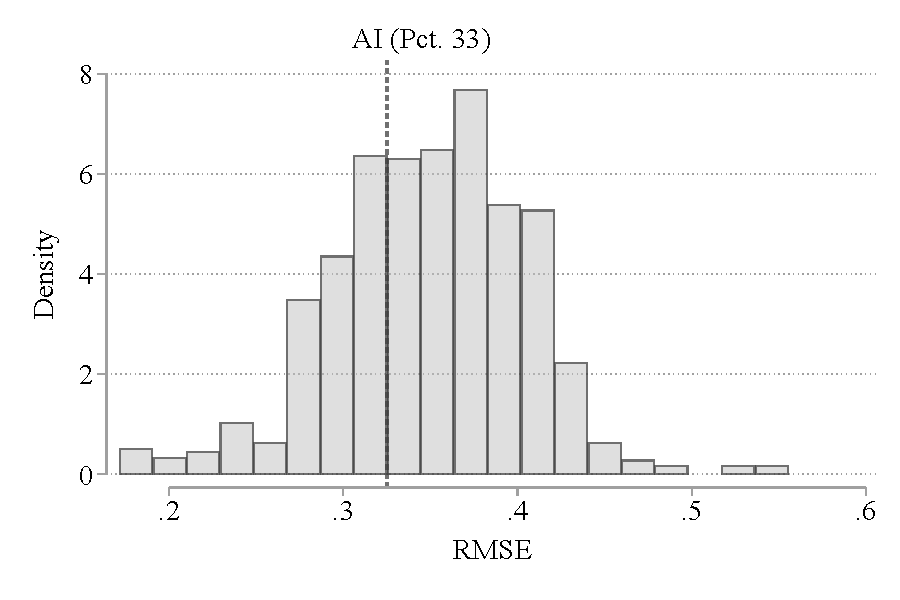
\includegraphics[width=7cm]{images/rmse_top_level_IN_NAI.pdf} }}%
    \qquad
    \subfloat[\centering AUROC Radiologists and AI]{{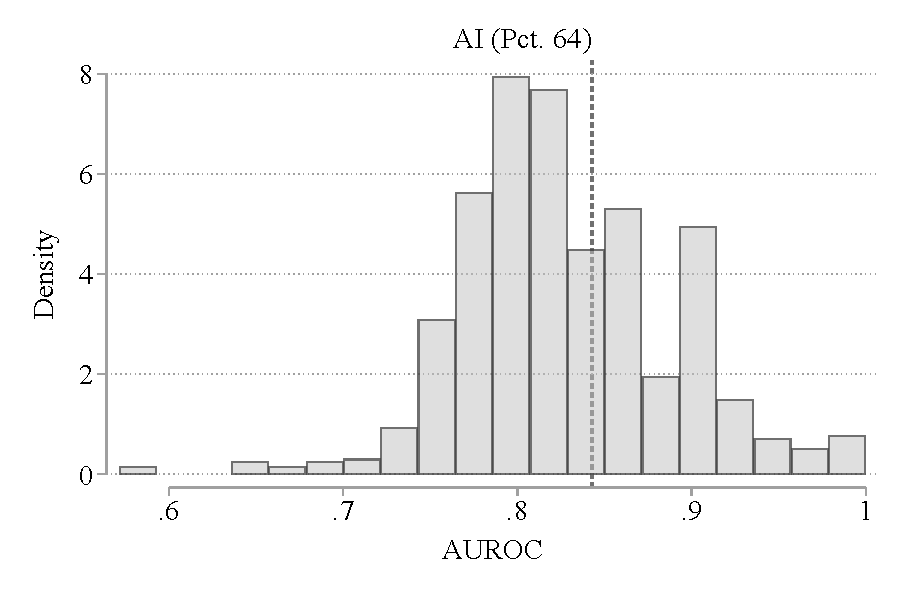
\includegraphics[width=7cm]{images/auroc_top_level_IN_NAI.pdf} }}%
\end{figure}
\begin{footnotesize}
  \noindent Note: These histograms show distributions of two different accuracy measures of radiologist assessments alongside the AI's accuracy. The left graph shows the distribution of the RMSE while the right shows the distribution of the average AUROC. Both distributions are shrunk to the grand mean using empircal Bayes. These measures are for each radiologist and include the top-level pathologies. The dotted line is the average measure of the AI algorithm for the corresponding distribution. Only the assessments where contextual history information is available for the radiologists but not the AI prediction are considered. 
\end{footnotesize}

\begin{figure}[H] 
\caption{AI Influence\label{fig:ai-influence}}
    \begin{center}
    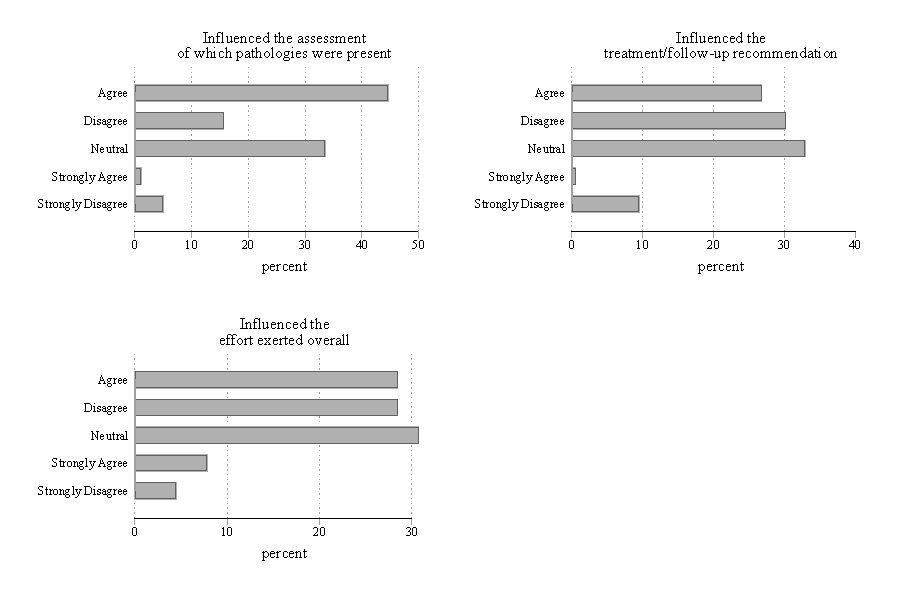
\includegraphics[width=0.8\textwidth]{images/ai_influence.pdf}
    \end{center}
\end{figure}

\begin{figure}[H]
    \caption{Clinical History Influence\label{fig:ch-influence}}
    \begin{center}
    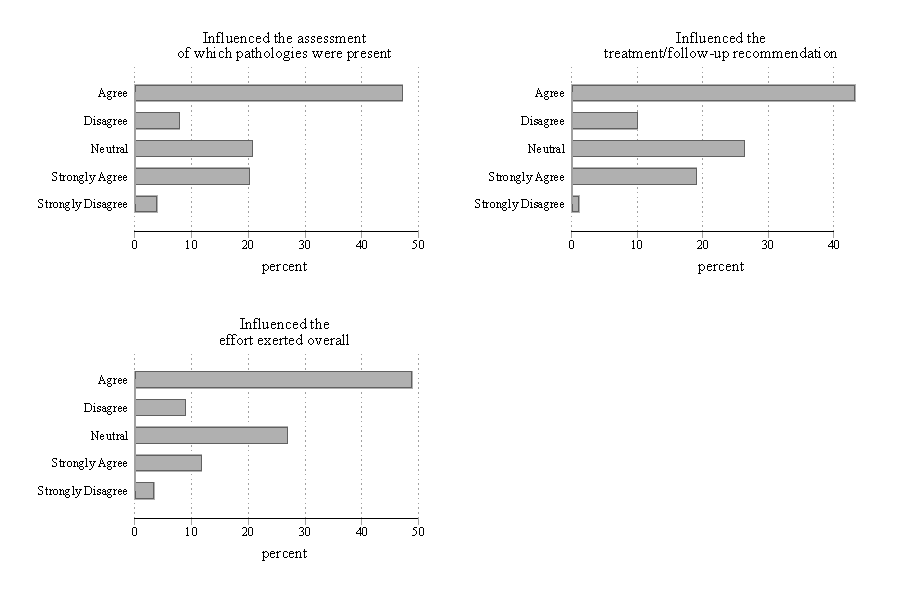
\includegraphics[width=0.8\textwidth]{images/ph_influence.pdf}
    \end{center}
\end{figure}